\chapter{Evaluation}
\label{ch:Evaluation}
This chapter aims to validate the hypotheses formulated for two distinct studies described in Chapter~\ref{ch:Design}. 
Each study focuses on specific aspects of ear-based temperature measurement and aims to explore the capabilities and limitations of the developed wearable prototype. 
For each study, a series of hypotheses have been put forward, and the data collected from the studies are used to evaluate these hypotheses.

\section{Results and Discussion from Study 1}
\label{sec:Evaluation:Study1}
Study 1 focuses on exploring the potential and limitations of the developed ear-based temperature measurement system, investigating its accuracy, reliability, and robustness under different conditions. 
A more detailed discussion of the design and goals of Study 1 is described in Chapter~\ref{ch:Design:Study:Study1}.

In Figure~\ref{fig:ch:Evaluation:Study1:RawData} an example measurement of participant 7 is shown.
To strengthen the insights obtained from this study, several hypotheses were formulated and tested. 
These hypotheses aim to address specific questions related to the performance and reliability of ear-based temperature measurements. 
The results and their implications are discussed in the subsequent sections, where each hypothesis is rigorously evaluated based on the collected data.

\begin{figure}[!h]
    \centering
    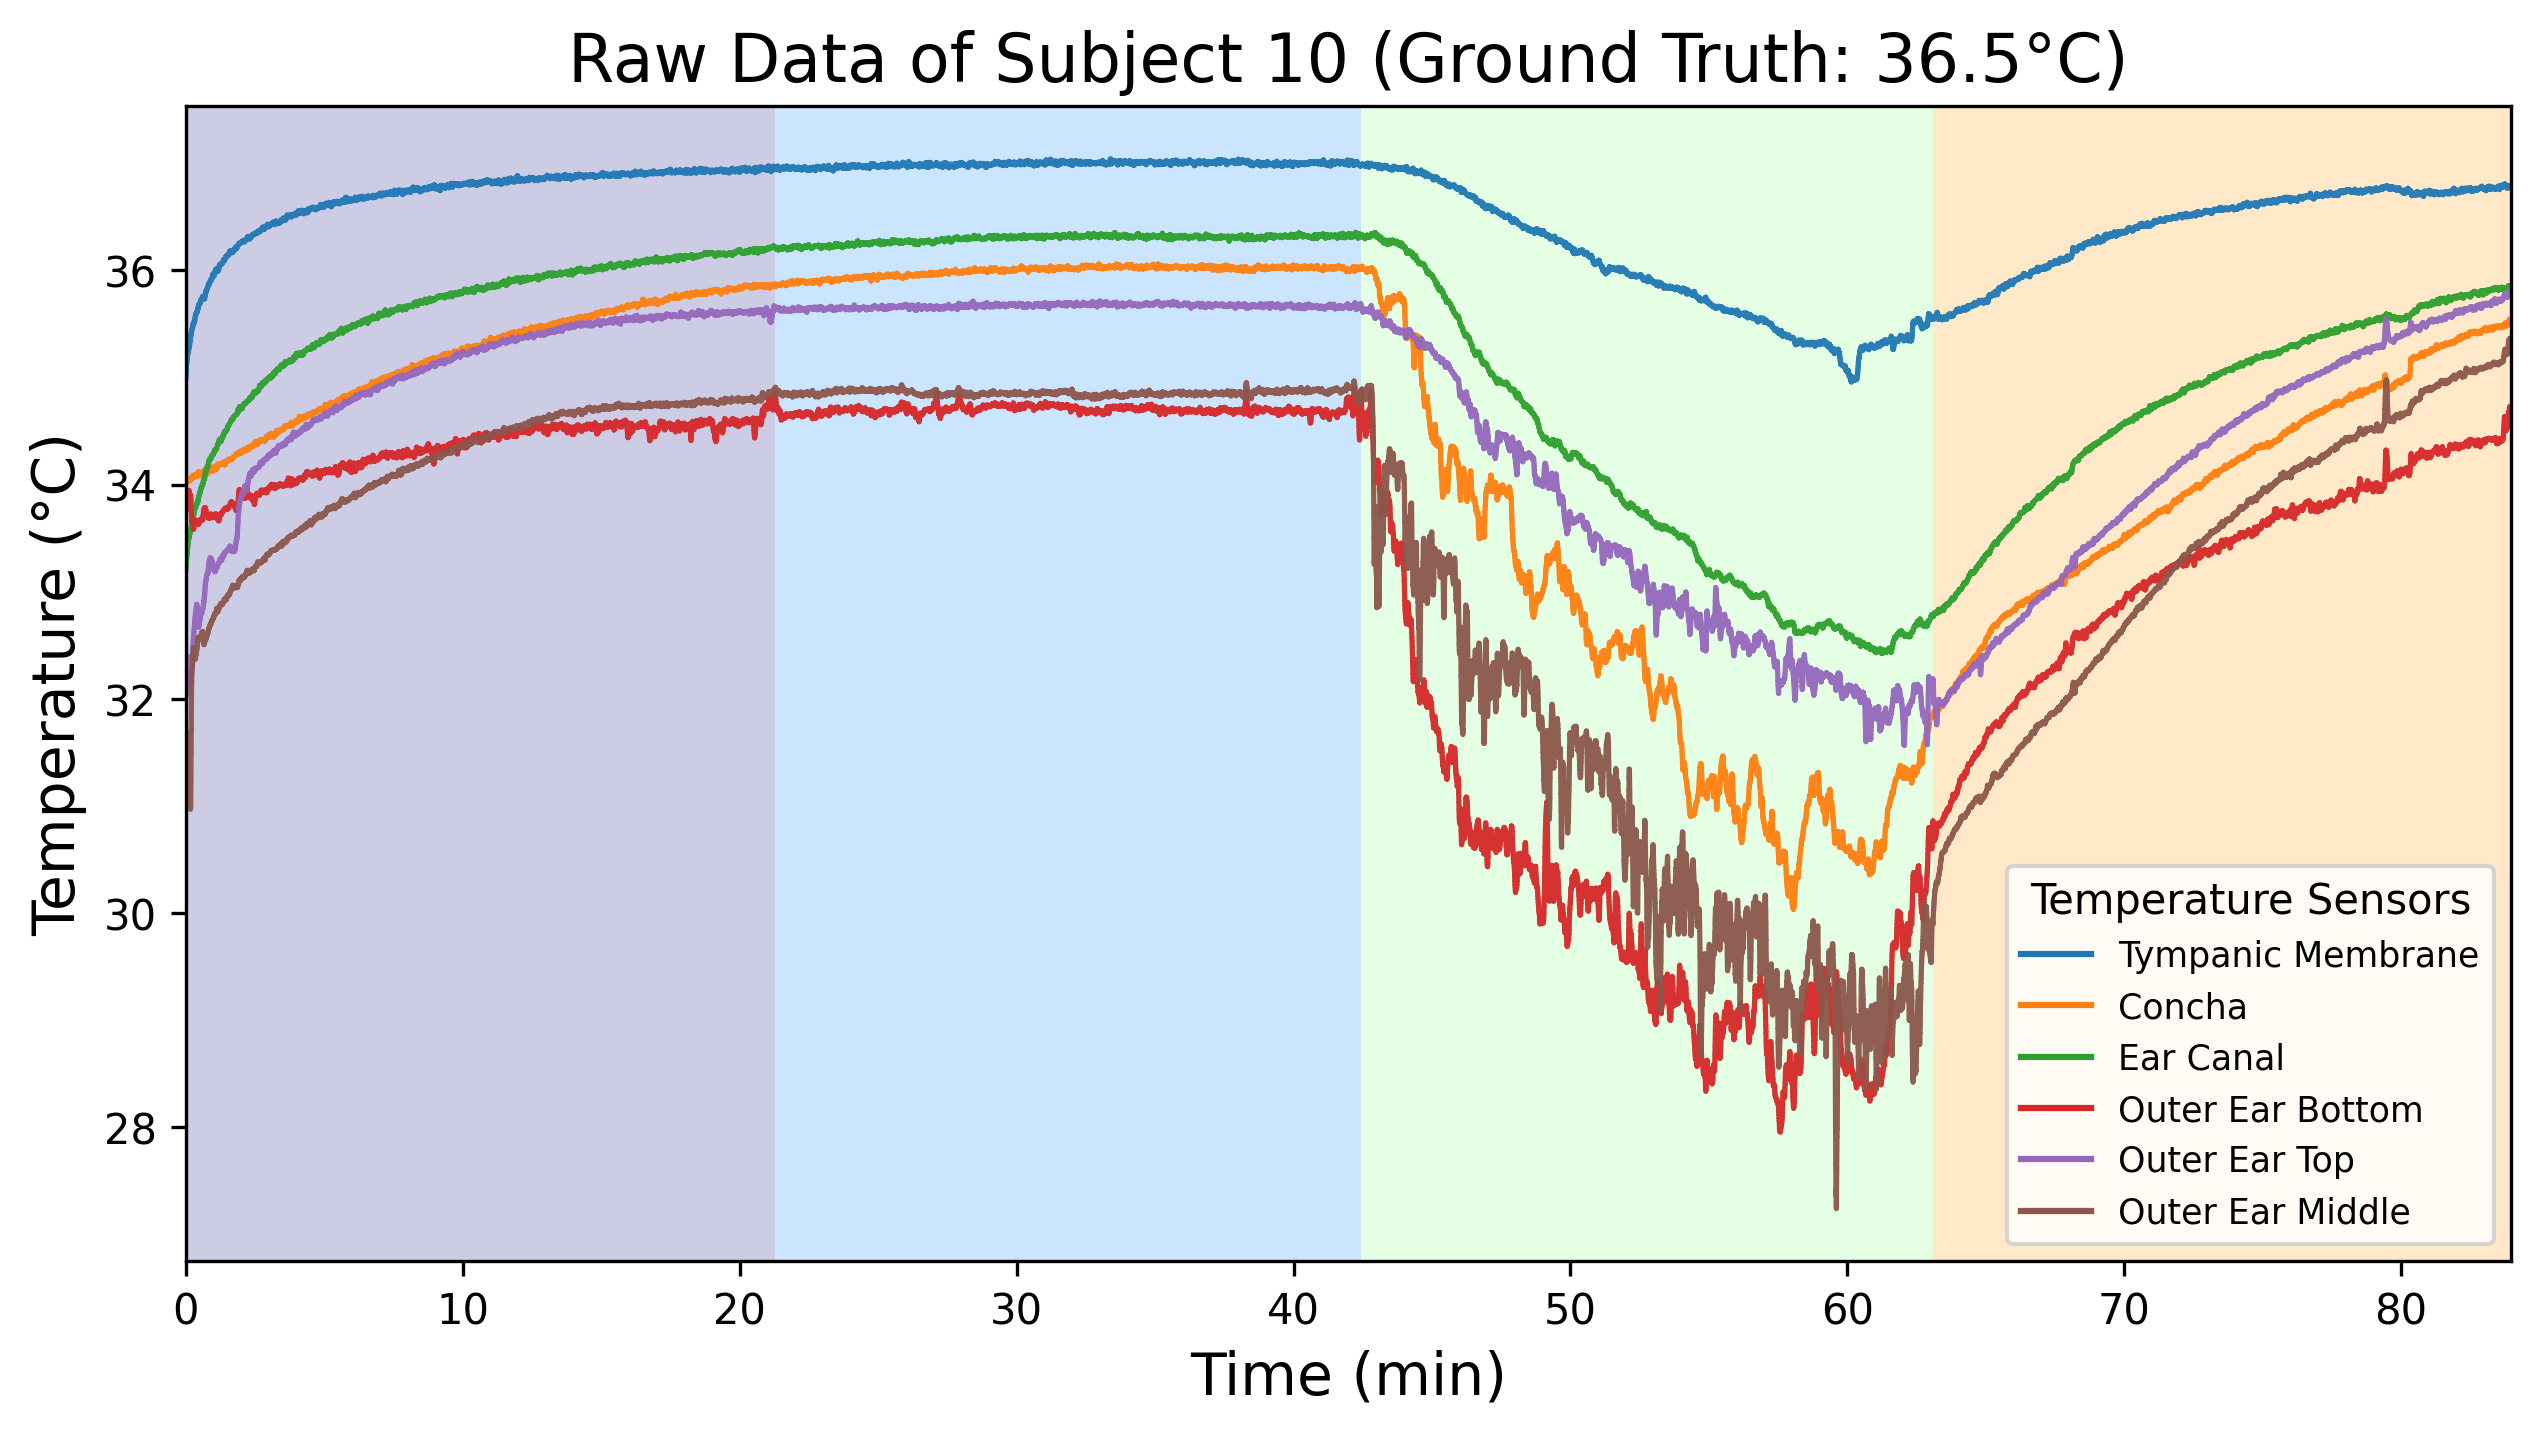
\includegraphics[width=\textwidth]{thesis-doc/images/study1/Logging_person_10_0smoothed_raw_data.png}
    \caption{Raw data of a measurement in study 1 of subject 10. The subject had a body temperature of $36.5^\circ\text{C}$ at the beginning. Phases 1-4 are shown, distinguished by the background color of the plot. In phase 1, the sensor has adjusted and acclimated to the temperature of the subject. After the sensor settled in, Phase 2 measured the temperature while sitting in a room. In phase 3, the subject went for a walk outside. In phase 4, he went back into the room to see how the sensors settled back to the calmer environmental conditions.}
    \label{fig:ch:Evaluation:Study1:RawData}
\end{figure}

\subsection{Hypothesis 1: Lower Temperature Measured on Sensors Behind the Ear}
\label{subsec:Evaluation:Study1:Hypothesis1}

The first hypothesis is to show that a lower temperature is measured behind the ear than in the ear.
For this purpose, the analysis was considered in two perspectives. 
First, only the data points where the subject was sitting were recorded, and second, all data were considered except for the acclimatization phase (phase 1).

In the first perspective, the data were considered at which the subject was seated (phase 2). 
Here, for all subjects, the mean temperature behind the ear was \(36.30^\circ\text{C}\), while the mean temperature inside the ear was \(36.74^\circ\text{C}\). 
To prove a statistically significant difference between the two means, a t-test can be used.
The t-test yielded a p-value of \(0.0424\), which is below the alpha value of \(0.05\).
Since the p-value is below the alpha, this is evidence of a significant difference.
The mean error between the ground truth and the temperature measured behind the ear was \(0.79^\circ\text{C}\), and that for the temperature in the ear was \(0.38^\circ\text{C}\). 
The p-value for the comparison of these errors was \(0.0115\), again indicating a statistically significant difference.
Thus, it is clear that temperature is measured significantly lower behind the ear than in the ear while sitting.

The second perspective now also looks at other phases of the study. 
Now, in addition to the sitting phase (phase 2), the walking phase (phase 3) and the regeneration phase (phase 4) were also considered. 
The mean temperature behind the ear was \(35.33^\circ\text{C}\) and in the ear it was \(36.02^\circ\text{C}\). 
The p-value of the T-test was \(0.0158\), which again is statistically significant.
The mean error behind the ear was \(1.67^\circ\text{C}\) and in the ear it was \(0.98^\circ\text{C}\). 
The p-value for the comparison of these errors was \(0.0158\), which is also statistically significant.

This can also be seen in Figure \ref{fig:eval:study1:hypothesis1_result}.
The two boxplot images show the sitting and walking phases (phase 2 and 3), always zeroed to the temperature measured by the thermometer before the measurement.
During sitting (phase 2), the temperature measured at the tympanic membrane is very close to the temperature measured by the thermometer ($\pm0.25^\circ\text{C}$). 
The sensors in the ear canal and pinna also show high accuracy. 
For the sensors behind the ear, although the median is sometimes very close to the sensors in the ear, the outliers are strongly represented here, which questions the reliability of the signals.
When comparing the sensors behind the ear, the sensor placed at the top behind the ear provides the best results. 
This is due to the position behind the ear, the further below the ear, the more external influences are felt, such as a gust of wind, even if only with slight movements.
This can be seen more clearly in the boxplot for phase 3, while the test subjects were out walking. 
While here also the sensor pointing to the eardrum shows the best results, all other sensors have outliers.
There is also a significant difference between the sensor in the ear canal and the auricle. 
The sensor in the ear canal is further in the ear and thus somewhat more protected from external conditions, which is also evident here. 
The findings of the boxplot from phase 2 are also confirmed for the sensors behind the ear.

The second perspective also confirms the hypothesis that the temperature measured behind the ear is statistically significantly lower than that measured in the ear. 
However, the sensors behind the ear also show a statistically significant higher error compared to the ground truth, especially when the subject is involved in activities such as walking. 
These findings have important implications for the use of ear-based temperature sensors in various applications.

\begin{figure}[!h]
    \centering
    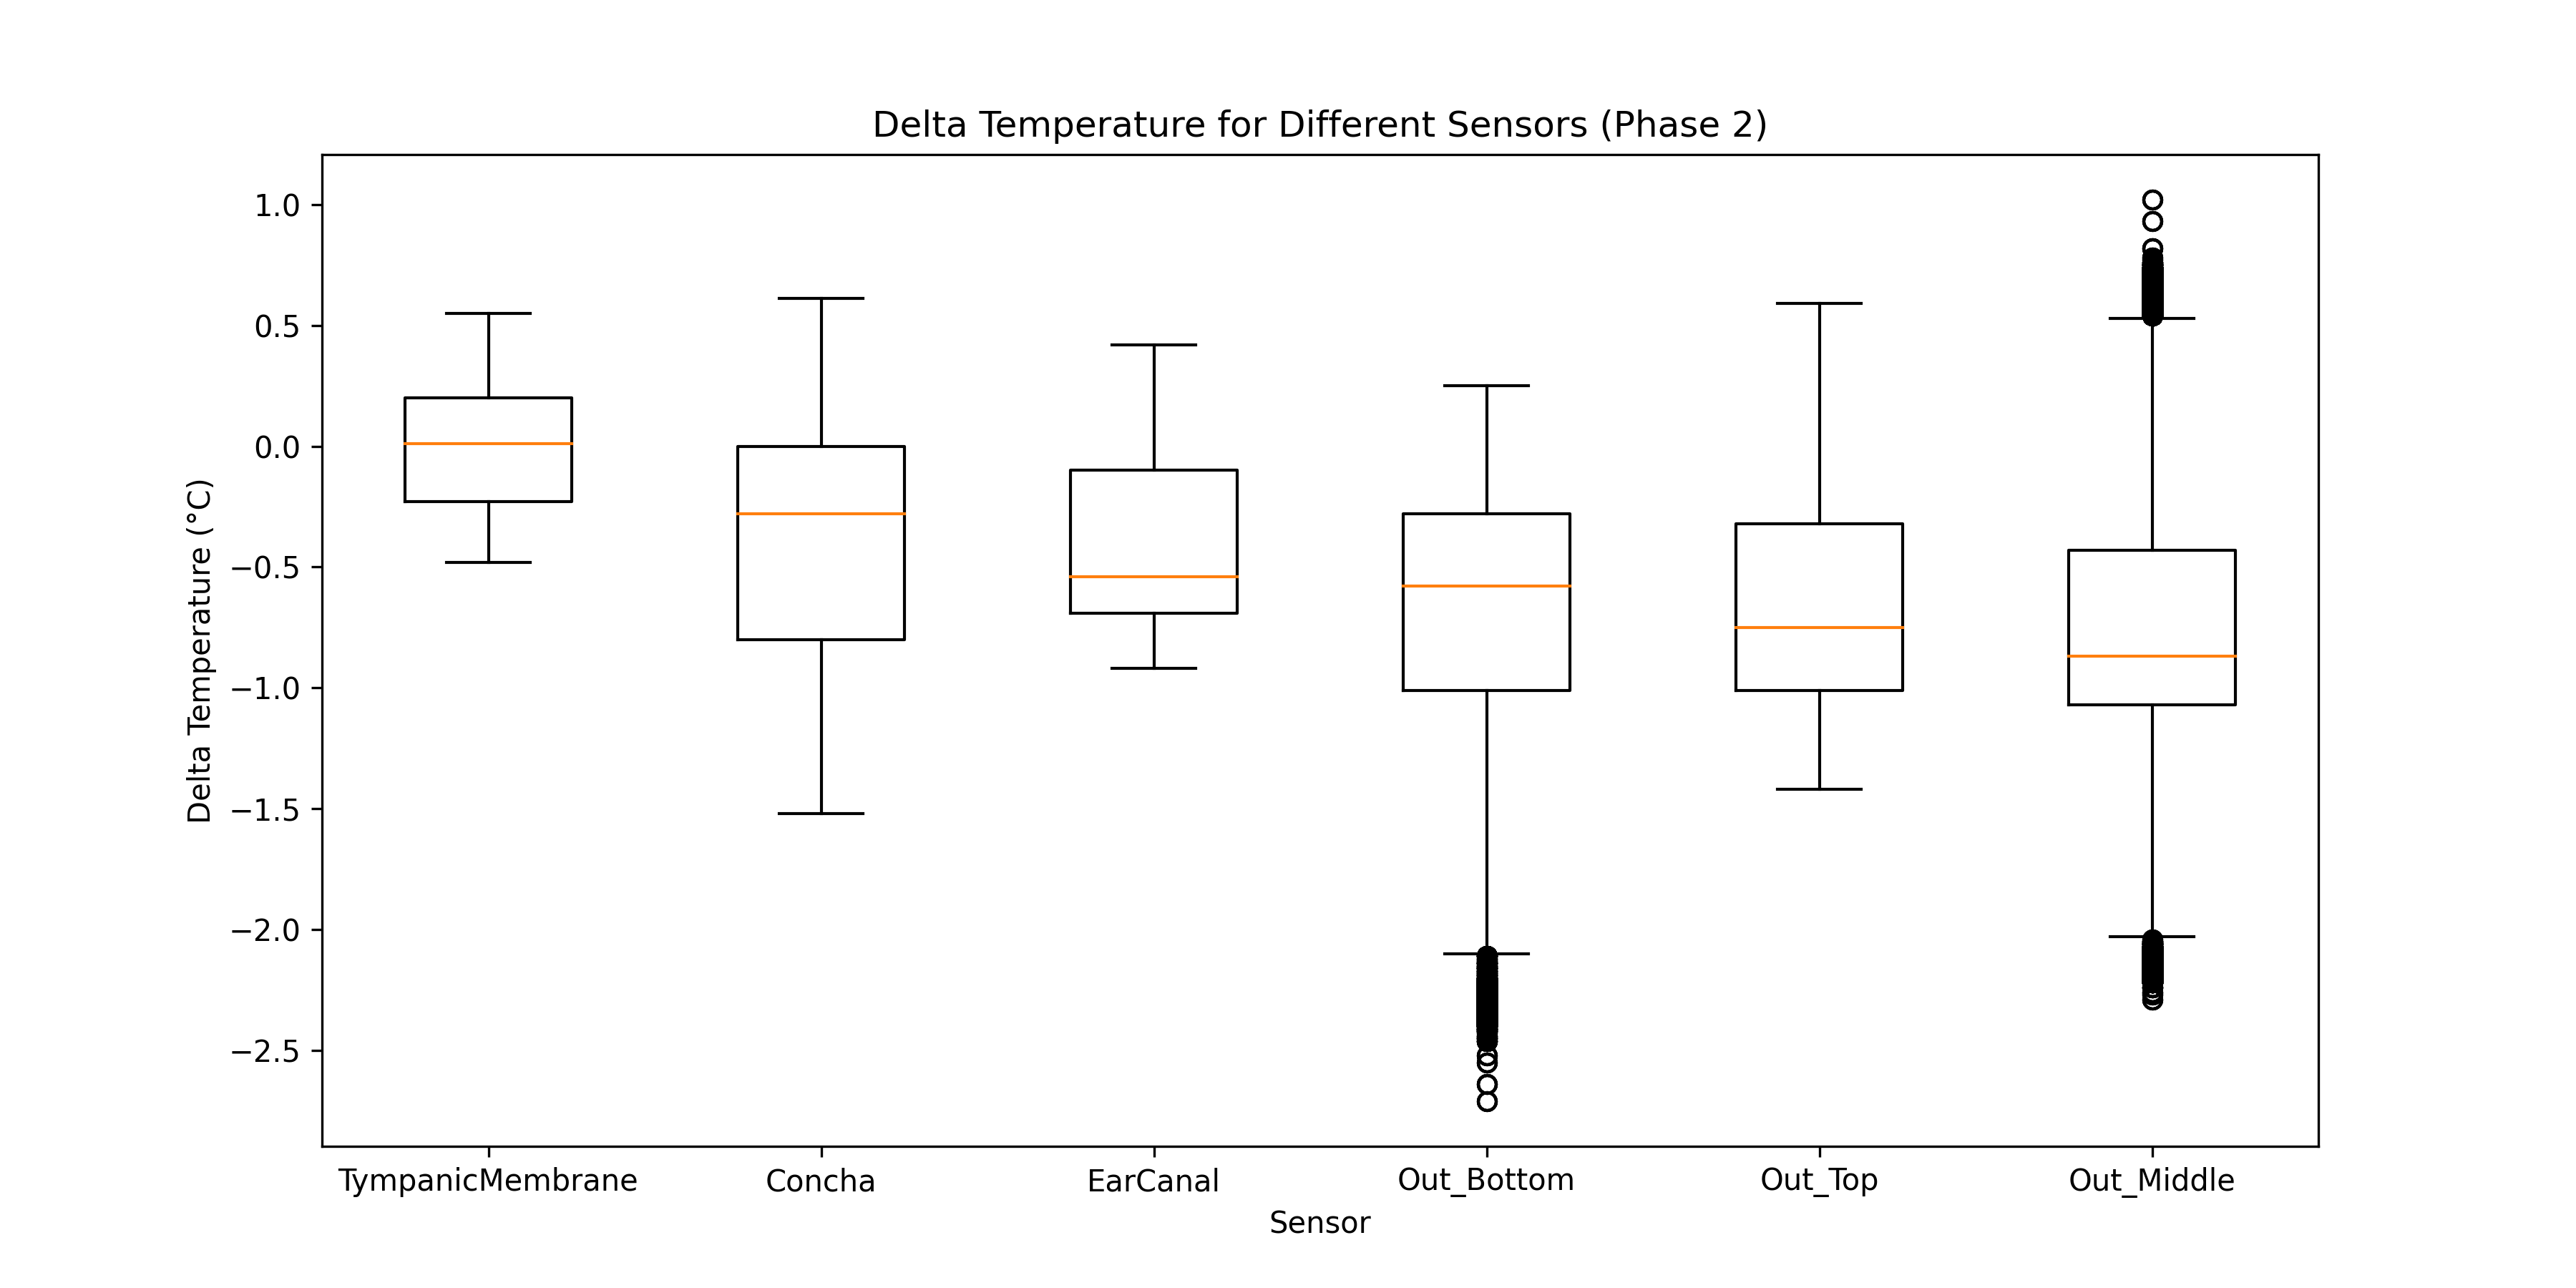
\includegraphics[width=\textwidth]{thesis-doc/images/study1/hypothesis1/hypothesis1_boxplot_phase_2.png}
    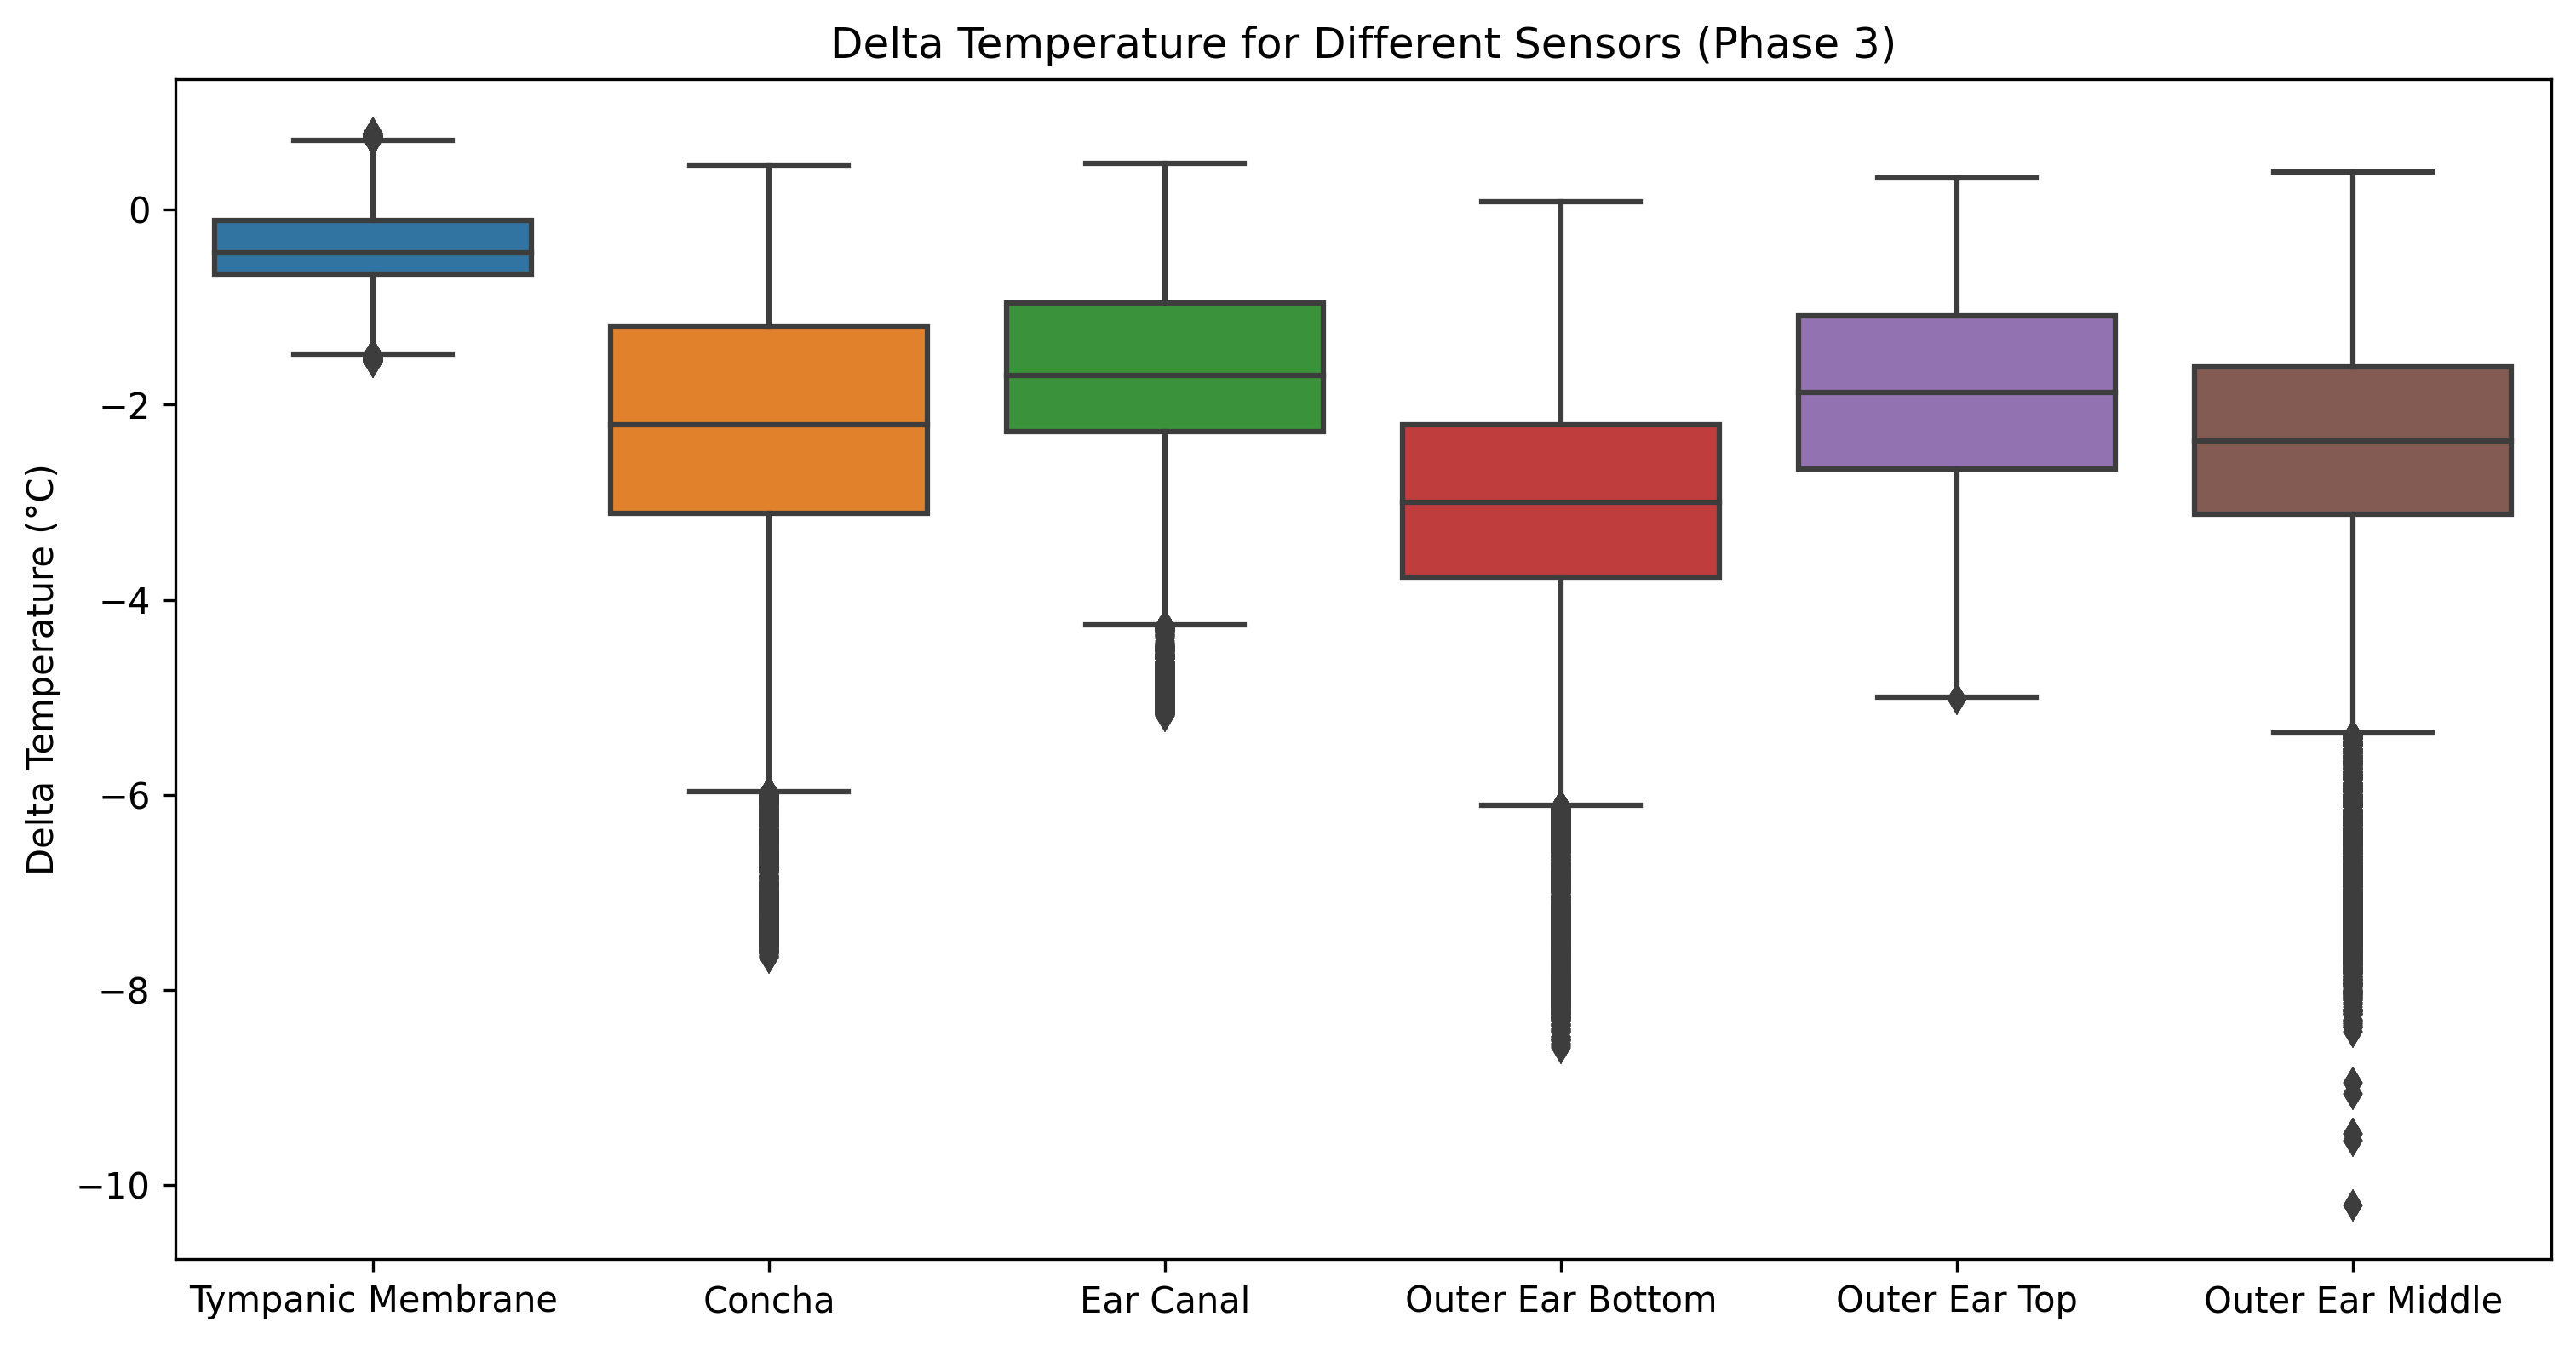
\includegraphics[width=\textwidth]{thesis-doc/images/study1/hypothesis1/hypothesis1_boxplot_phase_3.png}
    \caption{Boxplots visually illustrating the distribution of measured values from different sensor positions during phase 2 (indoor) and phase 3 (outdoor). Central tendencies and their dispersion for the analysis of the sensors under different environments can be seen. Temperature values were subtracted from the thermometer reading to compare all user data together. These visualizations are an essential part of the evaluation of Hypotheses 1 and 2, as they highlight differences in variance and highlight potential outliers.}
    \label{fig:eval:study1:hypothesis1_result}
\end{figure}

\subsection{Hypothesis 2: Variance Difference Indoor/Outdoor}
\label{subsec:Evaluation:Study2:Hypothesis2}

The second hypothesis is to show that the variance in temperature readings from ear-based sensors is lower indoors than outdoors.
This expectation is derived from the fact that the external influences in an indoor environment with closed windows are significantly less than the external influences outside during walking.
To test this hypothesis empirically, the data set of several ear-based temperature sensors at different positions was considered, both indoors and outdoors.
The different situations within the studies were divided into phases. 
Phase 2 represents an indoor measurement, and Phase 3 represents an outdoor measurement during walking.
Here, the temperature values in different areas of the ear were looked at closely.
To prove the hypothesis, the variances per temperature sensor were now calculated for phases 2 and 3 respectively. 
The results show a clear pattern. 
The mean variance for the tympanic sensor $0.00096$ indoors and \(0.107\) outdoors.
This pattern was consistently observed for other sensor locations, such as the auricle with a mean variance of $0.00307$ indoors and $1.134$ outdoors.
A detailed listing of the results can be seen in Table \ref{subsec:Evaluation:Study2:Hypothesis2:mean_variance_table}.
A two-sample T-test was used to statistically compare these variances.
The results provided clear evidence to support the hypothesis.
For example, the p-value for the tympanic sensor was significantly below the Bonferroni-corrected threshold, clearly refuting the null hypothesis.
This pattern is also seen for the other positions in and around the ear, providing extensive empirical support for the hypothesis.
In summary, the data confirm the second hypothesis: temperature measurements with ear-based sensors have significantly lower deviations when taken indoors than outdoors.

\begin{table}[t]
\centering
\begin{tabular}{|p{2.5cm}|c|c|c|c|c|c|}
\hline
Sensor & \multicolumn{2}{c|}{MAD (in \(^\circ\text{C}\))} & \multicolumn{2}{c|}{Mean Variance} & \multicolumn{2}{c|}{Mean Diff. from} \\
 & \multicolumn{2}{c|}{} & \multicolumn{2}{c|}{} & \multicolumn{2}{c|}{Ground Truth (in \(^\circ\text{C}\))} \\
\hline
 & Indoor & Outdoor & Indoor & Outdoor & Indoor & Outdoor \\
\hline
Tympanic Membrane & 0.025 & 0.258 & 0.00096 & 0.1074 & 0.0071 & -0.6077 \\
Concha & 0.042 & 0.820 & 0.00307 & 1.1339 & -0.3805 & -2.5609 \\
EarCanal & 0.030 & 0.624 & 0.00155 & 0.6456 & -0.3934 & -1.9584 \\
Out\_Bottom & 0.095 & 0.800 & 0.0189 & 1.1098 & -0.7439 & -3.3107 \\
Out\_Top & 0.062 & 0.663 & 0.00694 & 0.6499 & -0.6060 & -2.1198 \\
Out\_Middle & 0.101 & 0.831 & 0.0198 & 1.0982 & -0.7452 & -2.7643 \\
\hline
\end{tabular}
\caption{Mean absolute deviation (MAD), mean variance, and mean distance from ground truth for different sensors. Phases 2 (inside) and 3 (outside) were considered. All values were calculated for each sensor and averaged over all subjects.}
\label{subsec:Evaluation:Study2:Hypothesis2:mean_variance_table}
\end{table}

\subsection{Hypothesis 3: Relative Changes in Temperature Readings}
\label{subsec:Evaluation:Study1:Hypothesis3}
The third hypothesis examines the correlation between the relative changes in temperature readings from different sensor locations in Phases 2 and 3.
This is used to understand the consistency between the different sensor readings, particularly in relation to changing weather conditions.d
Mean absolute deviation is used for analysis to better understand the consistency between the different temperature sensor readings. 
Table \ref{subsec:Evaluation:Study2:Hypothesis2:mean_variance_table} shows the MAD value for each sensor location in phase 2 (indoor) and 3 (outdoor). 
Increased variance is seen in the outdoor phase. 
While the sensor measurement at the tympanic membrane is only $0.2 ^\circ\text{C}$, the other sensor locations have a mean absolute variance of about $0.6-0.8^\circ\text{C}$.
This is mainly due to the fact that external influences such as wind, rain, or sunlight may play a large role here.
When the subjects went for a walk, this was all represented, which explains the deviations here. 
This shows that these sensor positions are not as stable to external environmental influences as the sensor directed at the eardrum.
Similarly, this can be seen in the heatmap of Figure \ref{fig:eval:study1:hypothesis3_result}. 
Here, the correlations in phase 2 (indoor) and phase 3 (outdoor) have been plotted as a heatmap. 
Significant differences in the correlation of temperature values between the two phases 2 and 3 can be seen. 
In phase 2, the correlations are generally slightly lower, especially the measurement of tympanic membrane is very different from the other results.
This can be explained by variations in the subjects' sensor results, for example, when subjects readjust the sensor or move their head awkwardly, especially for the sensors behind the ear. 
In contrast, the correlations in Phase 3 are higher than average, often exceeding $0.9$. 
This suggests that all sensors respond equally to external environmental changes.
The reason for this is that during outdoor activities, conditions such as wind and sunlight affect all sensor locations equally.
This explains the sharp drop in temperature readings, resulting in high correlations.
In summary, the heat map supports the hypothesis by showing that indoor sensor readings fluctuate widely, while outdoor conditions tend to synchronize readings, albeit with higher volatility.
In summary, this hypothesis is supported by the analysis of the mean absolute deviation. 
Furthermore, it can be seen that the sensors at the different positions are differently stable to external environmental influences, especially when the subjects are outdoors.

\begin{figure}[t]
    \centering
    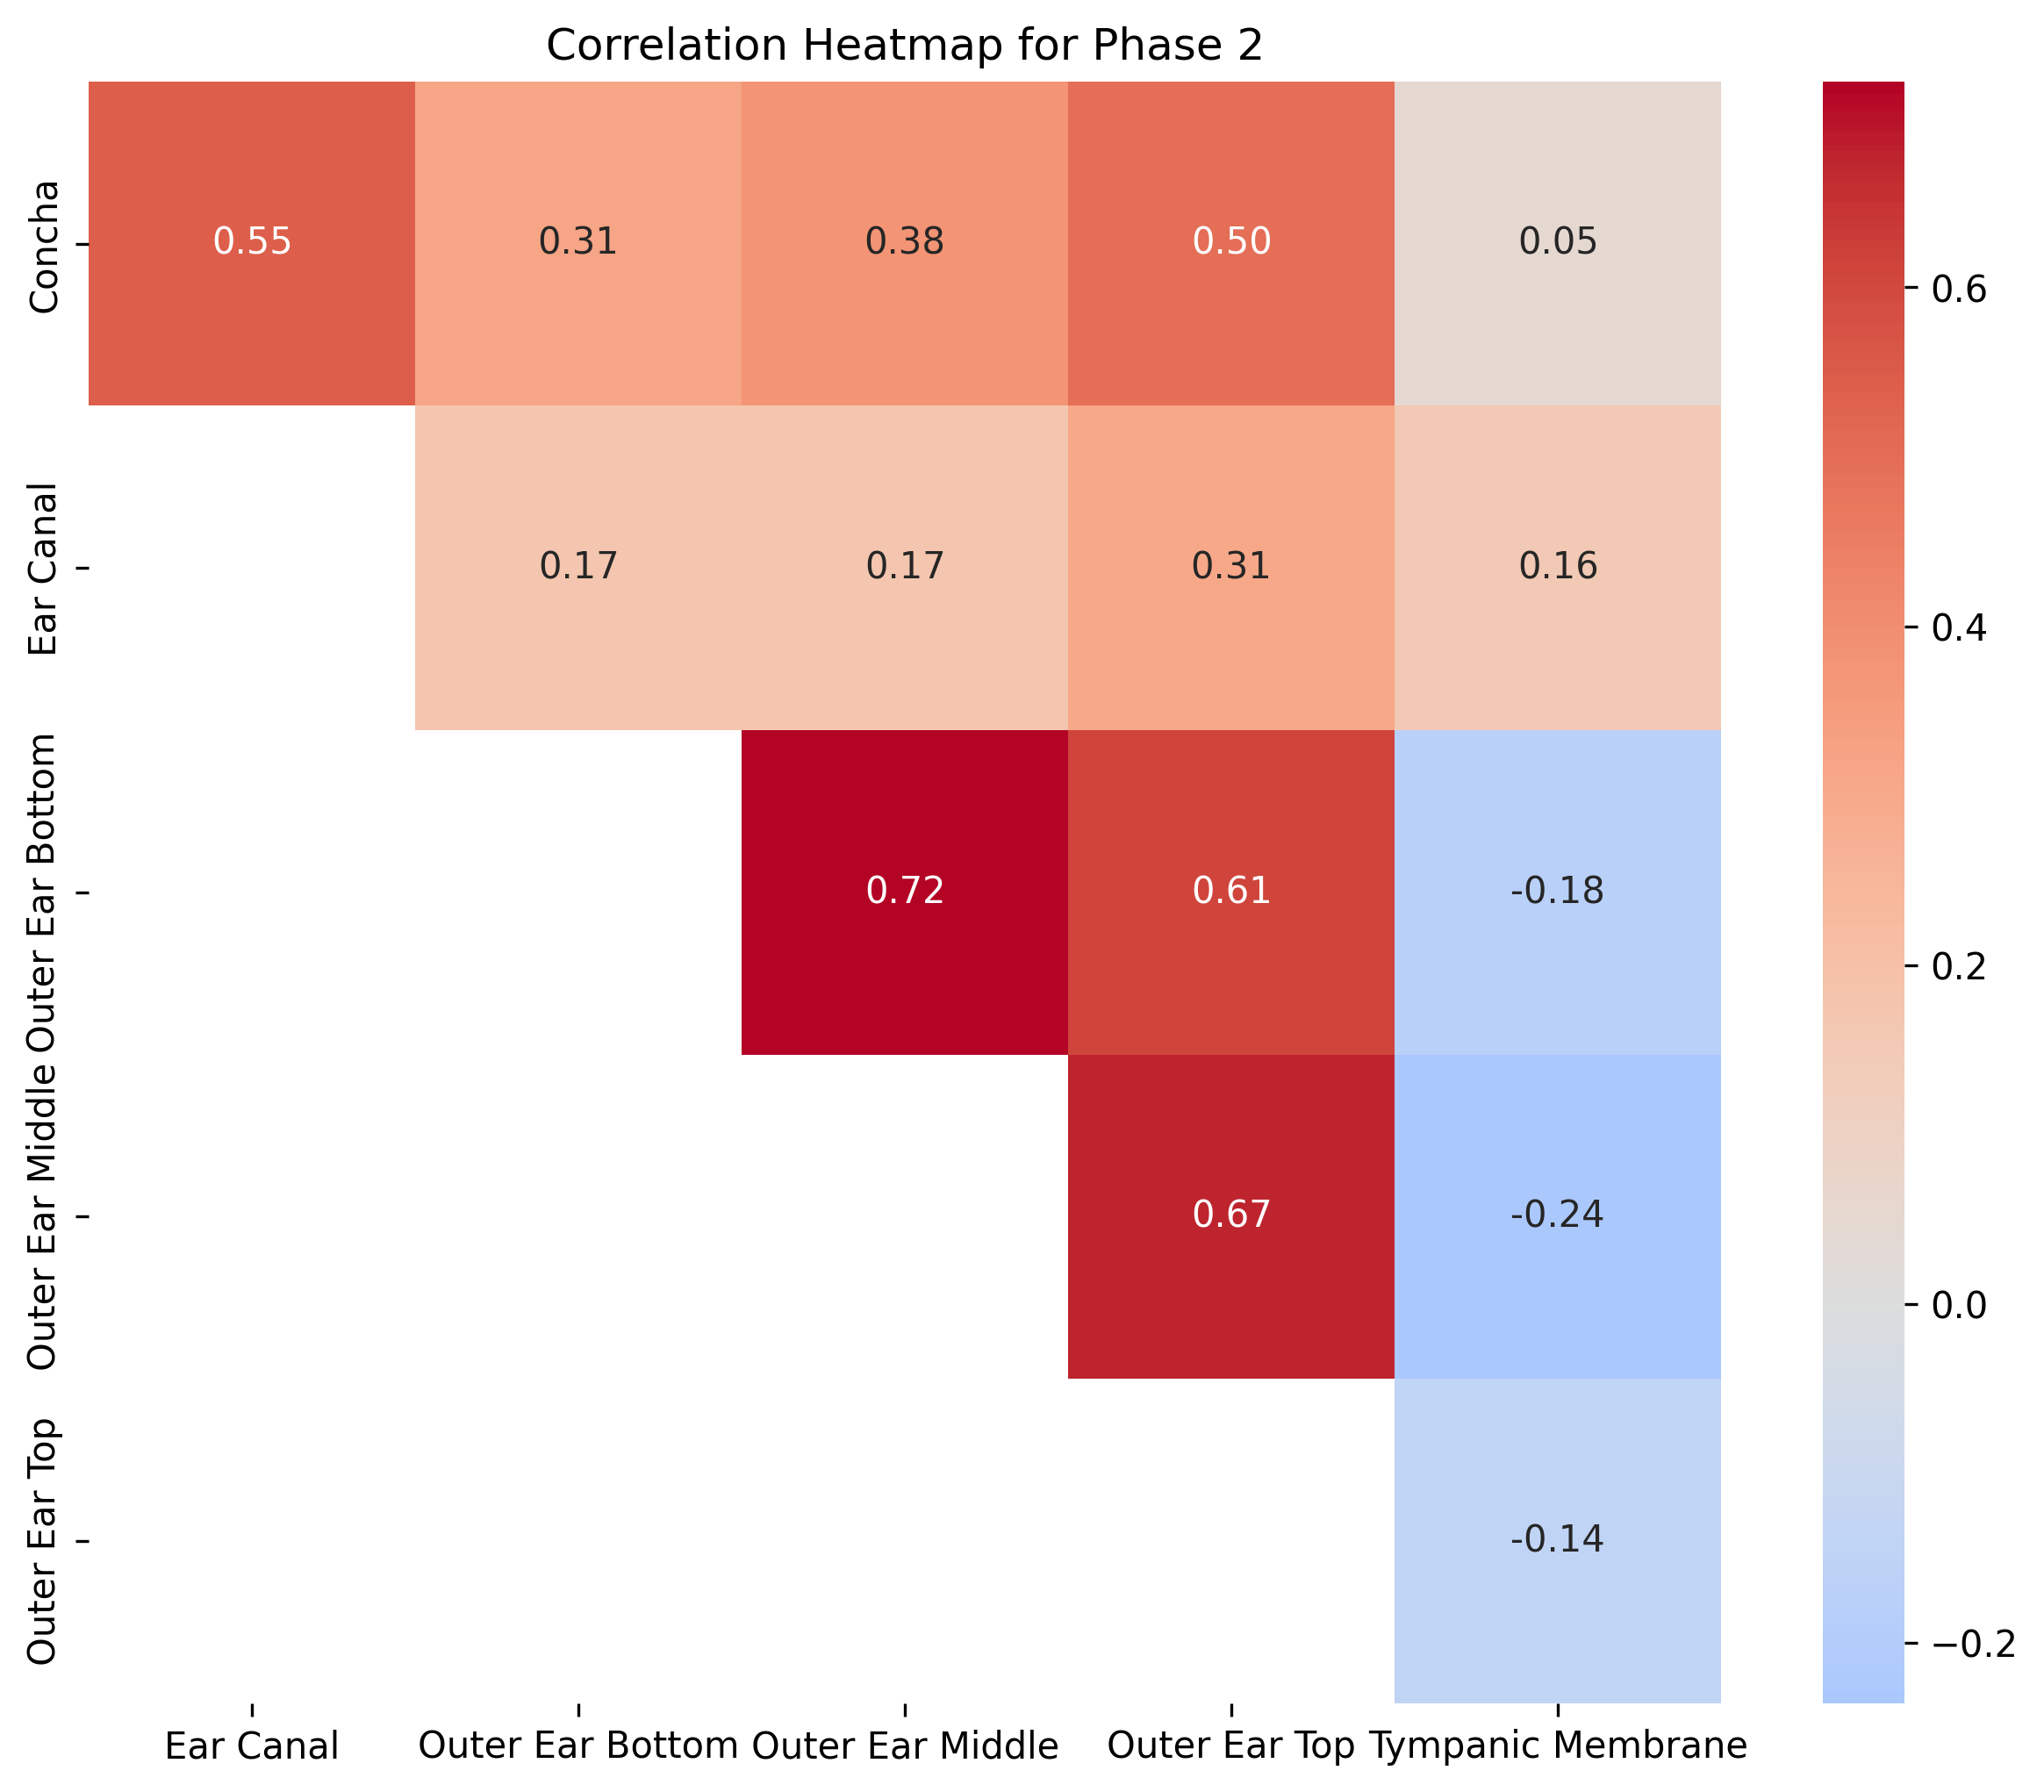
\includegraphics[width=0.9\textwidth]{thesis-doc/images/study1/hypothesis3/Correlation_Heatmap_Phase_2.png}
    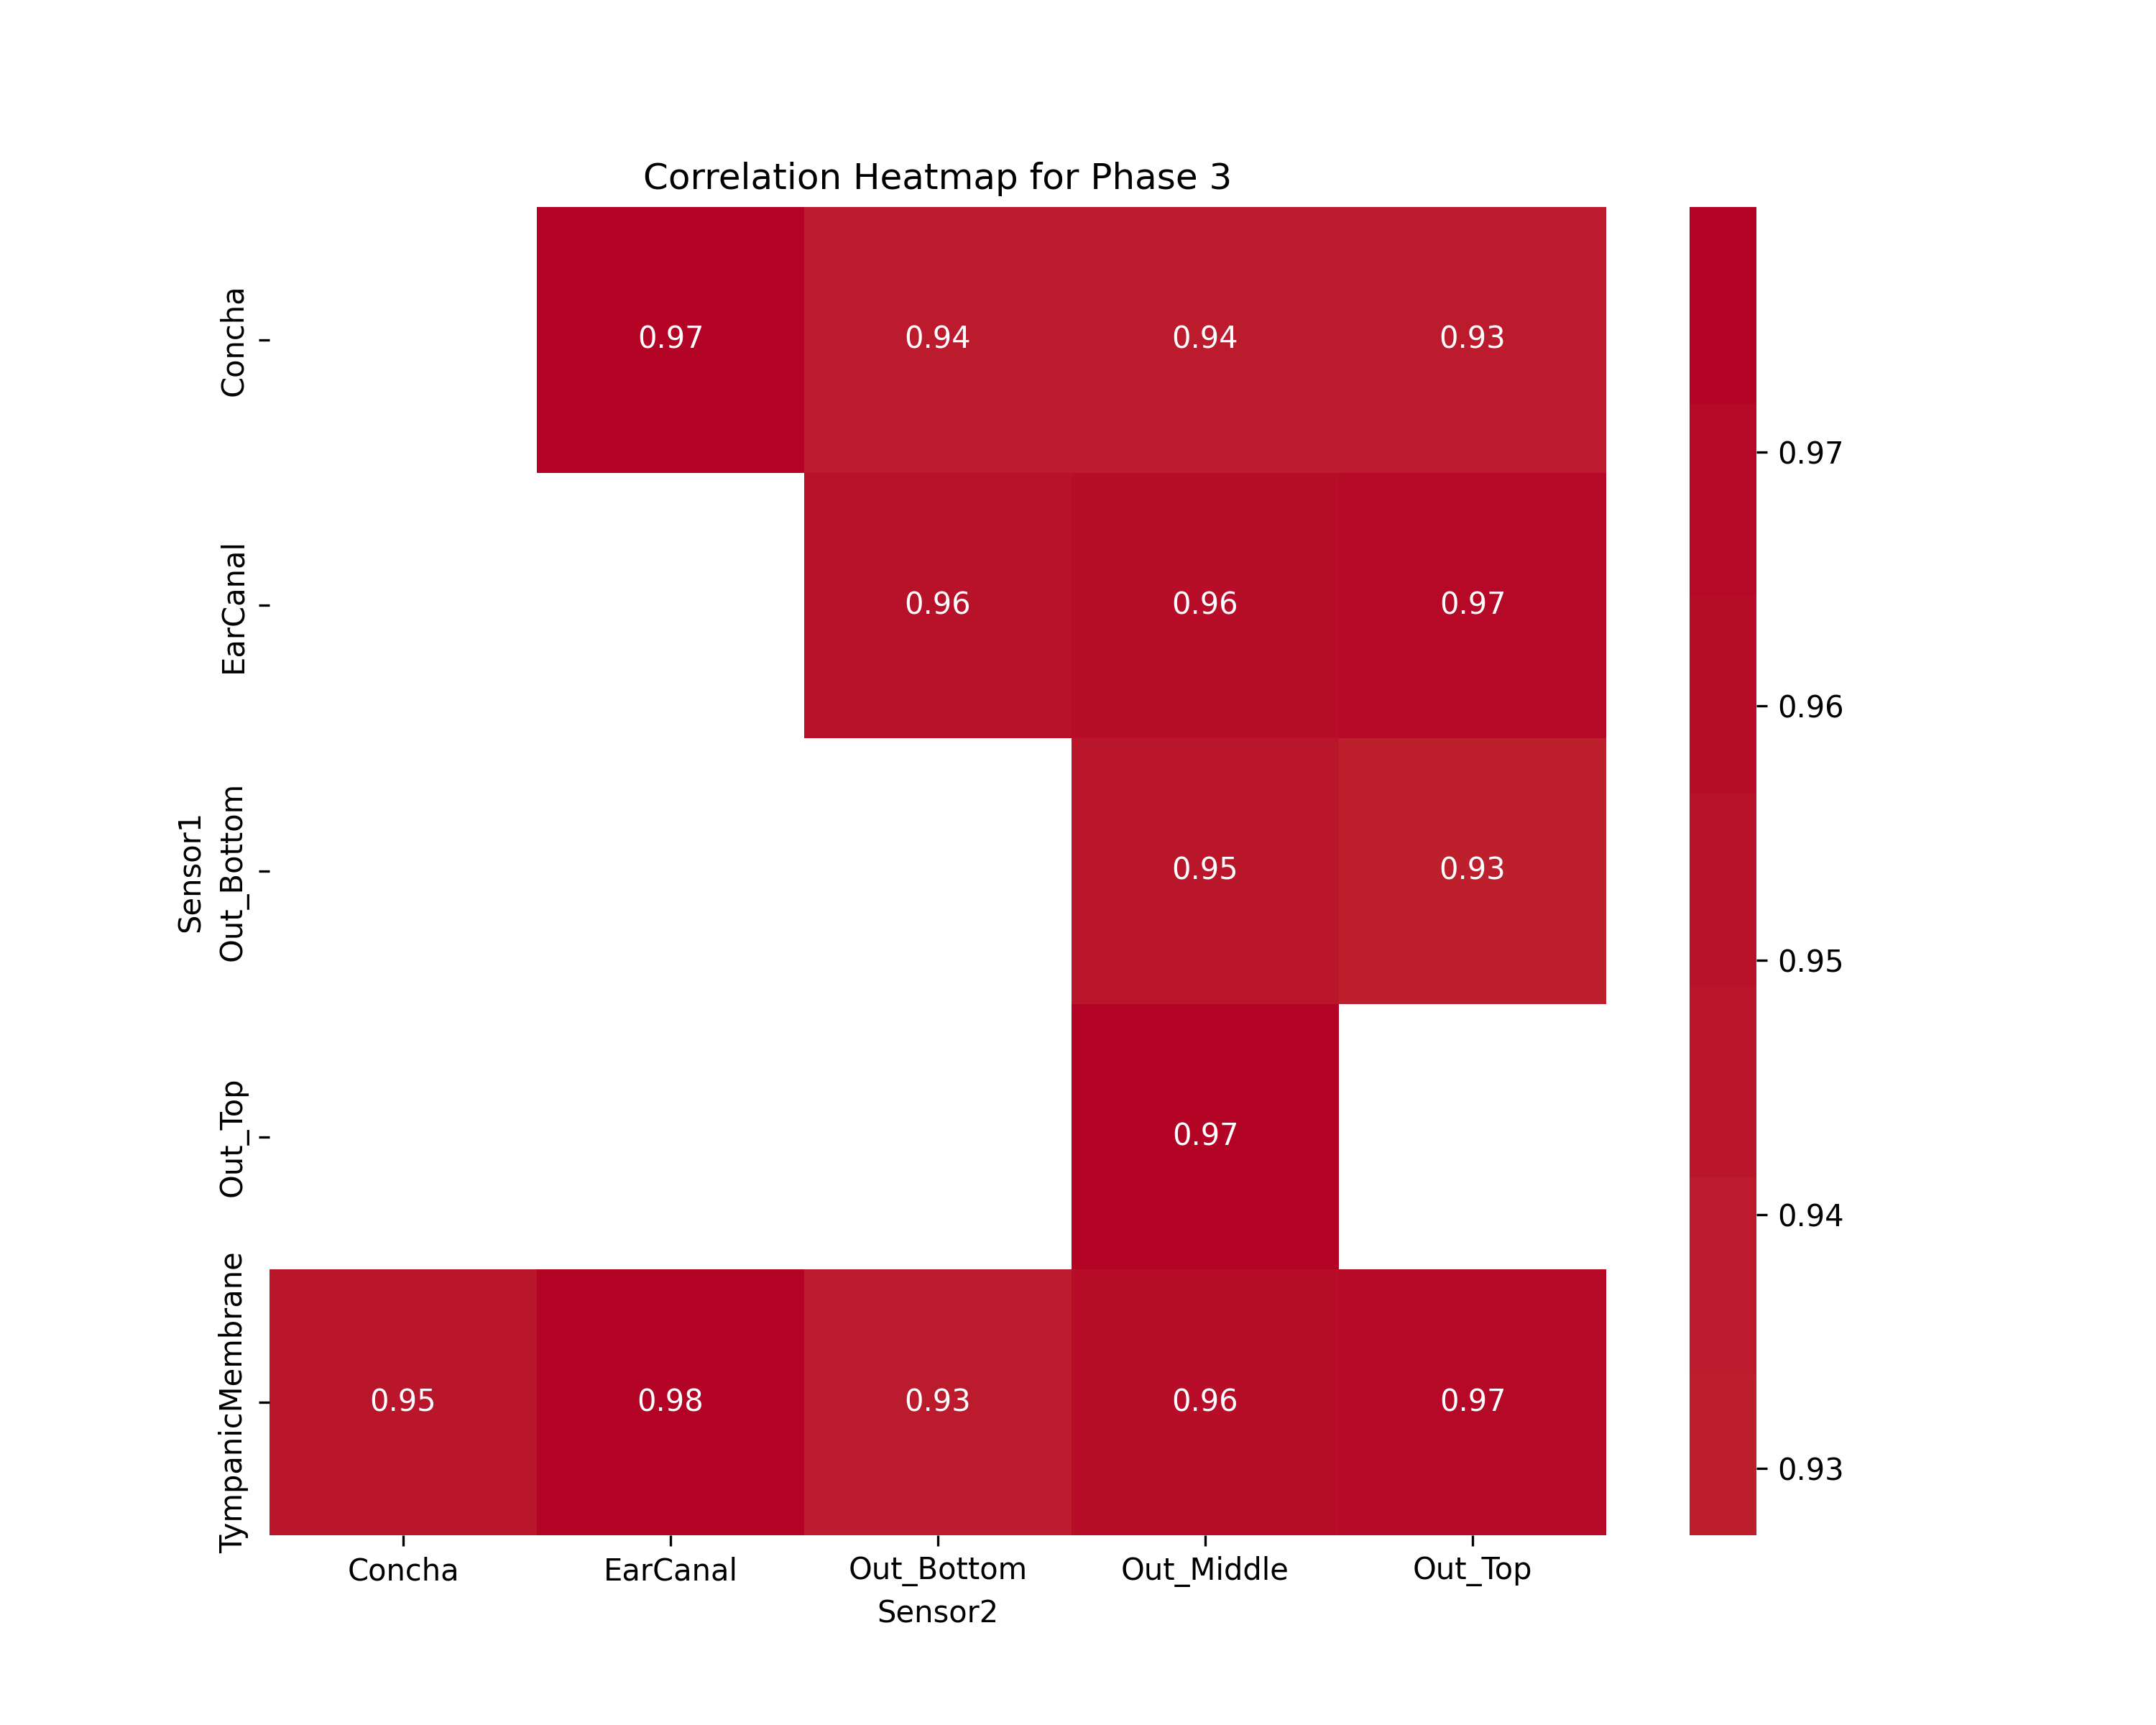
\includegraphics[width=0.9\textwidth]{thesis-doc/images/study1/hypothesis3/Correlation_Heatmap_Phase_3.png}
    \caption{Heat maps showing the correlation matrices of temperature readings from different ear-based sensors during Phase 2 (indoor) and Phase 3 (outdoor). The color-coded matrices provide a visual representation of how strongly each pair of sensors correlates under different conditions. Darker shading represents higher correlation and helps assess consistency between sensor measurements and their sensitivity to environmental changes, providing empirical evidence for Hypothesis 3.}    
    \label{fig:eval:study1:hypothesis3_result}
\end{figure}

\subsection{Hypothesis 4: Temperature at the Tympanic Membrane Is Most Stable}
\label{subsec:Evaluation:Study1:Hypothesis4}
The fifth hypothesis considers the stability of temperature sensor readings at the tympanic membrane compared to other positions during phases 2 (indoor) and 3 (outdoor).
The metric used here is the standard deviation. 
The standard deviation results can be found in Table \ref{subsec:Evaluation:Study1:Hypothesis4:std_dev_table}. 
In phase 2, the standard deviation is still relatively similar for all measurements, with only the position behind the ear in the middle yielding a worse value of $0.1154$. 
The standard deviation from the tympanic membrane nevertheless sets itself apart from those of the others with $0.0288$ compared to $0.05-0.07$. 
In phase 3, however, it is clear that the measurement of temperature at the tympanic membrane shows the most stability. 
At $0.1971$, the deviation is significantly smaller than for the rest $0.65-0.92$. 
Additionally, it can be seen from the figure \ref{fig:eval:study1:hypothesis1_result} that measurements at the tympanic membrane shows the least quantile differences and is closest to the thermometer values. 
From the calculated standard deviations, it appears that the tympanic membrane has the lowest values in both phases, indicating higher stability. 
In contrast, the other sensors show higher standard deviations, more specifically the sensors outside the ear. 
This makes them more susceptible to external conditions, such as environmental changes.
Thus, this confirms the hypothesis that the pom-pom skin provides the most stable temperature readings.

\begin{table}[t]
\centering
\begin{tabular}{|l|c|c|}
\hline
Sensor & Mean Standard Deviation & Mean Standard Deviation \\
& Phase 2 (indoor) & Phase 3 (outdoor) \\
\hline
Tympanic Membrane & 0.0308 & 0.3048 \\
Concha & 0.0535 & 0.9882 \\
Ear Canal & 0.0378 & 0.7496 \\
Out\_Bottom & 0.1138 & 1.0156 \\
Out\_Top & 0.0730 & 0.7836 \\
Out\_Middle & 0.1176 & 0.9875 \\
\hline
\end{tabular}
\caption{Standard deviations of temperature readings for different sensors during phases 2 and 3, averaged over all subjects. Lower values indicate higher stability.}
\label{subsec:Evaluation:Study1:Hypothesis4:std_dev_table}
\end{table}

\subsection{Hypothesis 5: Movement Leads to Changes in the Temperature Readings}
\label{subsec:Evaluation:Study1:Hypothesis5}

Hypothesis 5 states that the physical movement of the participants will have an effect on the various temperature sensors. 
This section will cover the methodology, evaluation, and discussion of this hypothesis.
To investigate the influence of exercise, both phases 2 and 3 were considered. 
In phase 2, subjects sat in a room for 20 minutes, and in phase 3, they walked outdoors for 20 minutes.
During both phases, temperature was measured at the 6 temperature sensors using $8 Hz$. 
In addition, data from the inertial measurement unit (IMU), which consists of an accelerometer, a gyroscope, and a magnetometer, were sampled at $50Hz$. 
The relative change was now calculated for each temperature sensor as follows:

\[
\text{relative change} = \left| \frac{{T_{\text{current}} - T_{\text{previous}}}}{{T_{\text{previous}}}} \right| \times 100
\]

Where \( T_{\text{current}} \) and \( T_{\text{previous}} \) are the current and previous temperature values, respectively. 
The absolute value of the relative change was taken to capture the magnitude of the change regardless of direction. 
This value was then multiplied by 100 to express it as a percentage.
In addition, the mean motion was derived from the IMU data.
For this purpose, a metric for mean motion was calculated. 
For each time point, the mean motion \(M\) was calculated using the following formula:

\[
M = \sqrt{{\sum_{i=1}^{n} x_i^2}}
\]

Where \( x_i \) is the IMU reading from one of the 9 columns (`ACC\_X`, `ACC\_Y`, `ACC\_Z`, `GYRO\_X`, `GYRO\_Y`, `GYRO\_Z`, `MAG\_X`, `MAG\_Y`, `MAG\_Z`). This approach effectively captures the total motion intensity at each time point by considering all available IMU sensors.
Figure \ref{fig:eval:study1:hypothesis5_result} shows the relative changes in each temperature sensor reading for the indoor and outdoor phases.
The movement of the subjects is shown at the bottom. 
The plots show a nuanced relationship between movement and temperature sensor values.
Relative changes can be seen for the individual temperature sensors in the two phases, but this may be due to different conditions. 
In Phase 3, temperature generally decreased significantly when subjects left the room and went outside.
This is exacerbated by movement during the outdoor phase. 

\begin{figure}[t]
    \centering
    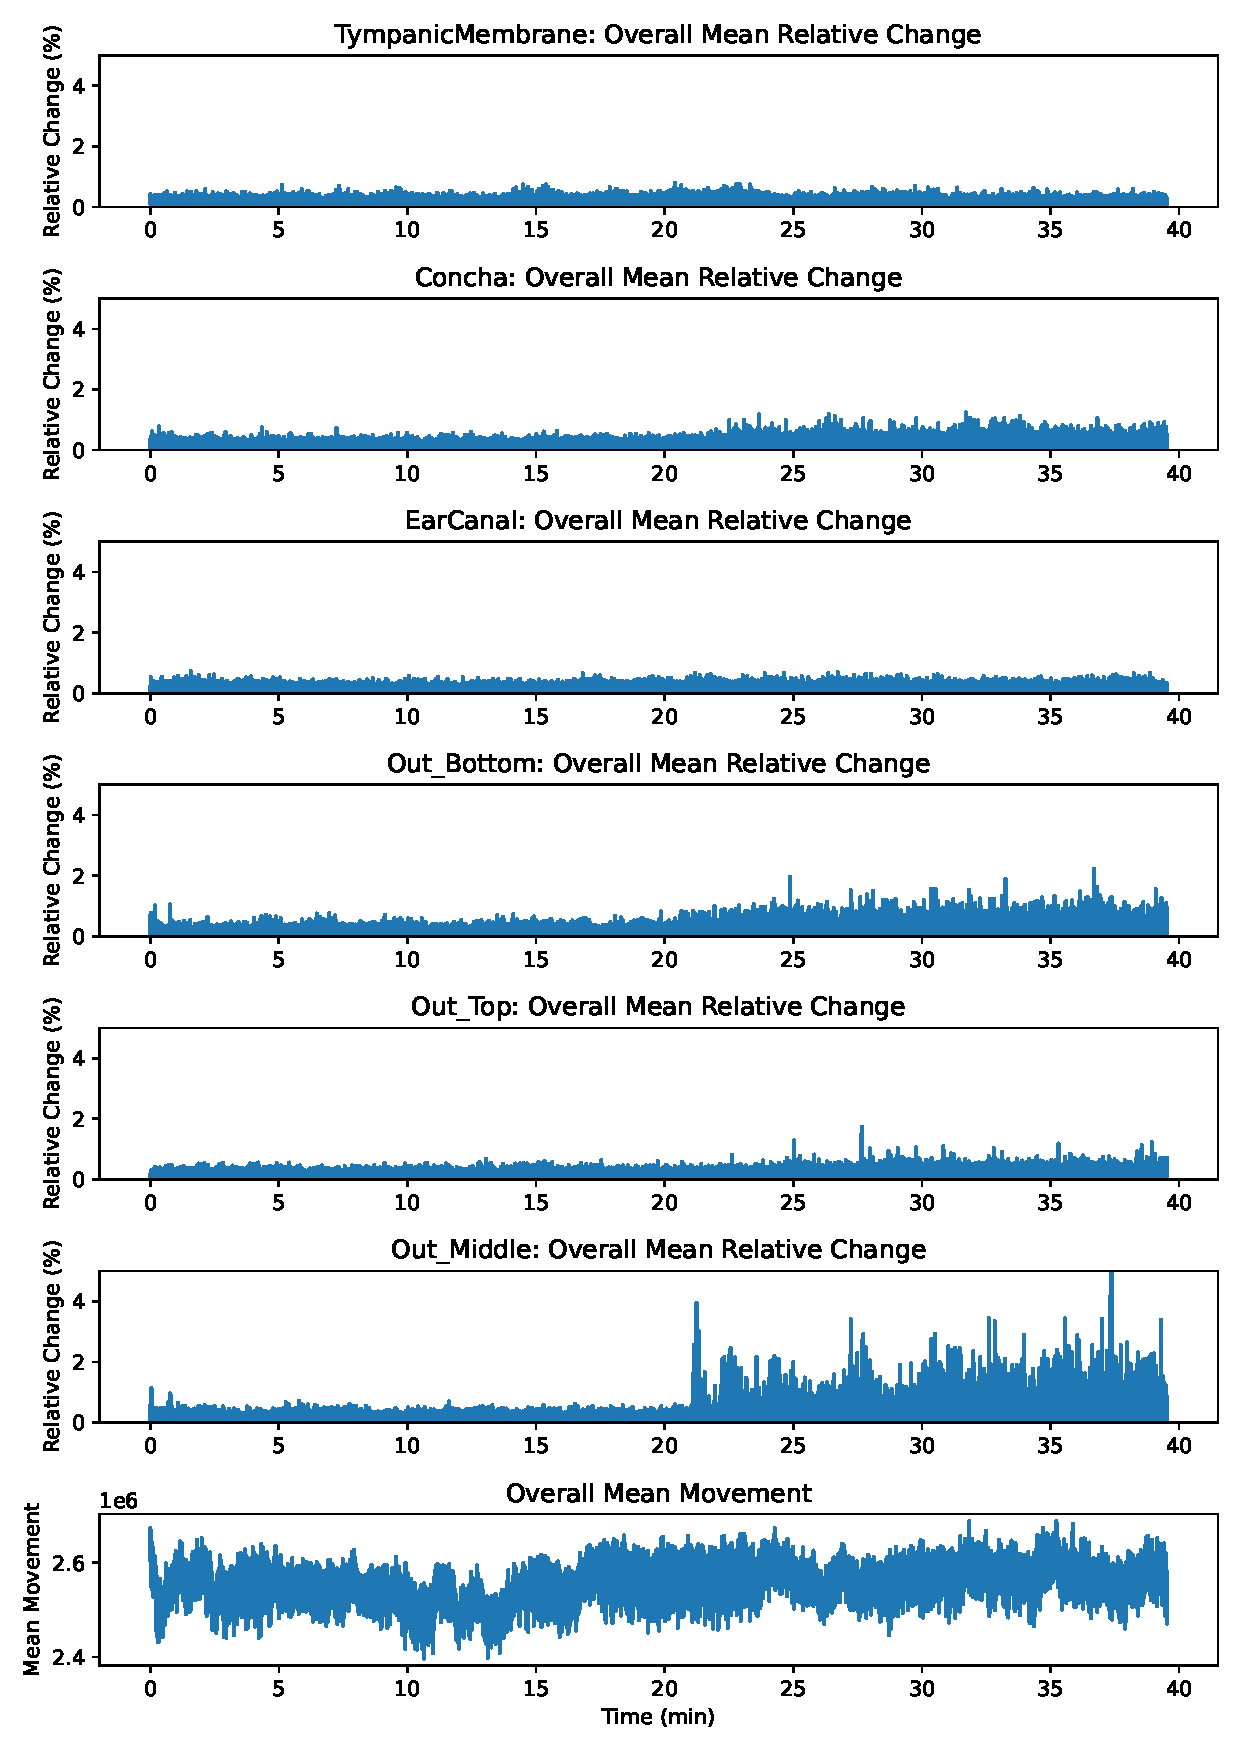
\includegraphics[width=\textwidth]{thesis-doc/images/study1/hypothesis5/overall_mean_data_hypothesis5.pdf}
    \caption{ADD DESCRIPTION}    
    \label{fig:eval:study1:hypothesis5_result}
\end{figure}


\section{Results and Discussion from Study 2}
\label{sec:Evaluation:Study2}
Having checked the validity of the temperature measurements, a second study will now observe how the measured temperature behaves when the subject is placed under stress.
A more detailed introduction to the design and objectives of study 2 is described in chapter~\ref{ch:Design:Study:Study2}.

\subsection{Hypothesis 1: ...}
\label{subsec:Evaluation:Study2:Hypothesis1}
asdf

\subsection{Hypothesis 2: ...}
\label{subsec:Evaluation:Study2:Hypothesis2}
asdf

\subsection{Hypothesis 3: ...}
\label{subsec:Evaluation:Study2:Hypothesis3}
asdf

\subsection{Hypothesis 4: ...}
\label{subsec:Evaluation:Study2:Hypothesis4}
asdf

\subsection{Hypothesis 5: ...}
\label{subsec:Evaluation:Study2:Hypothesis5}
asdf